\section{Resultados Experimentales}

A continuación se presentan los resultados obtenidos tras ejecutar la suite de pruebas.

\subsection{Tiempo de Ejecución}
La Figura \ref{fig:tiempo} muestra el tiempo de ejecución en escala logarítmica respecto al número de animes $n$.

\begin{figure}[H]
    \centering
    % 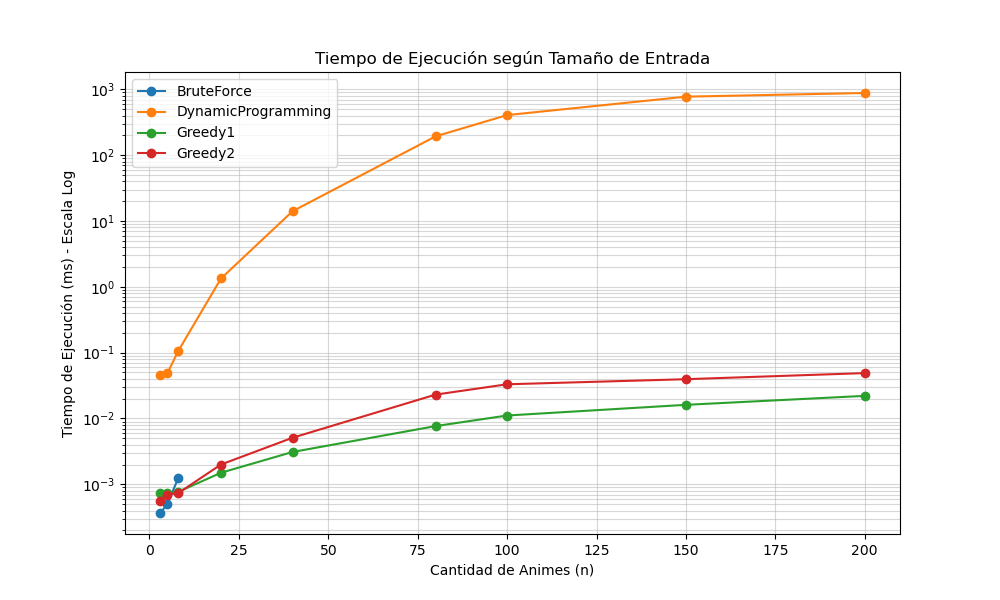
\includegraphics[width=0.8\textwidth]{../code/implementation/data/plots/tiempo_vs_n.png}
    \caption{Tiempo de ejecución promedio por algoritmo.}
    \label{fig:tiempo}
\end{figure}

Se observa que la Programación Dinámica crece de manera lineal respecto a $n$, lo cual es consistente con su complejidad teórica $O(n \cdot M \cdot E \cdot q)$. Las heurísticas Greedy son órdenes de magnitud más rápidas, manteniendo tiempos casi instantáneos incluso para $n=200$.

\subsection{Uso de Memoria}
La Figura \ref{fig:memoria} presenta el consumo de memoria máximo durante la ejecución.

\begin{figure}[H]
    \centering
    % 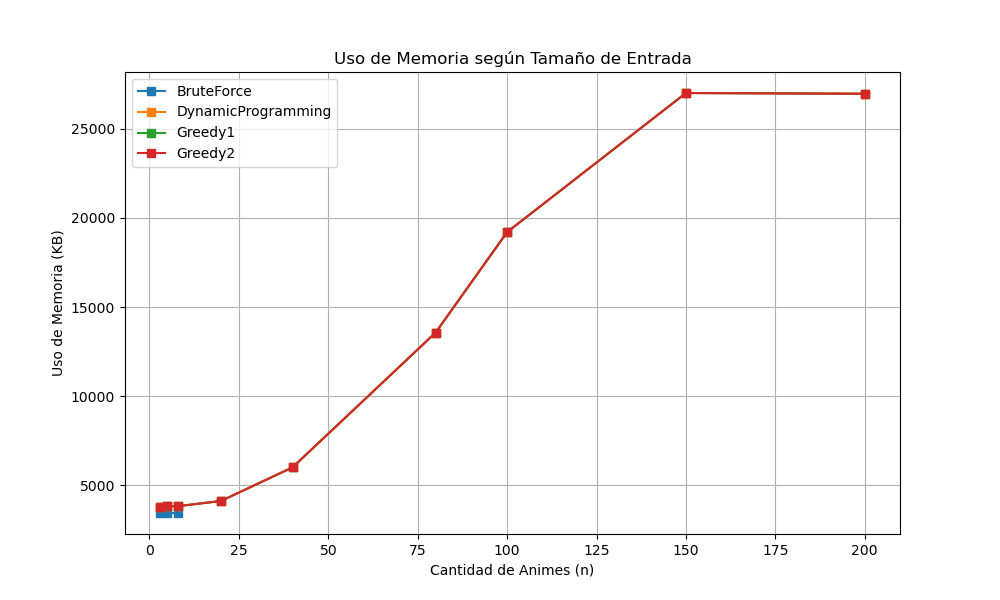
\includegraphics[width=0.8\textwidth]{../code/implementation/data/plots/memoria_vs_n.png}
    \caption{Uso de memoria máximo por algoritmo.}
    \label{fig:memoria}
\end{figure}

El uso de memoria de DP se mantiene constante una vez que la matriz de $3000 \times 500$ es reservada. Las variaciones menores observadas en los gráficos corresponden a las estructuras de datos que almacenan la instancia del problema.

\subsection{Calidad de la Solución}
La calidad se define como el ratio entre la satisfacción de Greedy y la de DP (óptima).

\begin{figure}[H]
    \centering
    % 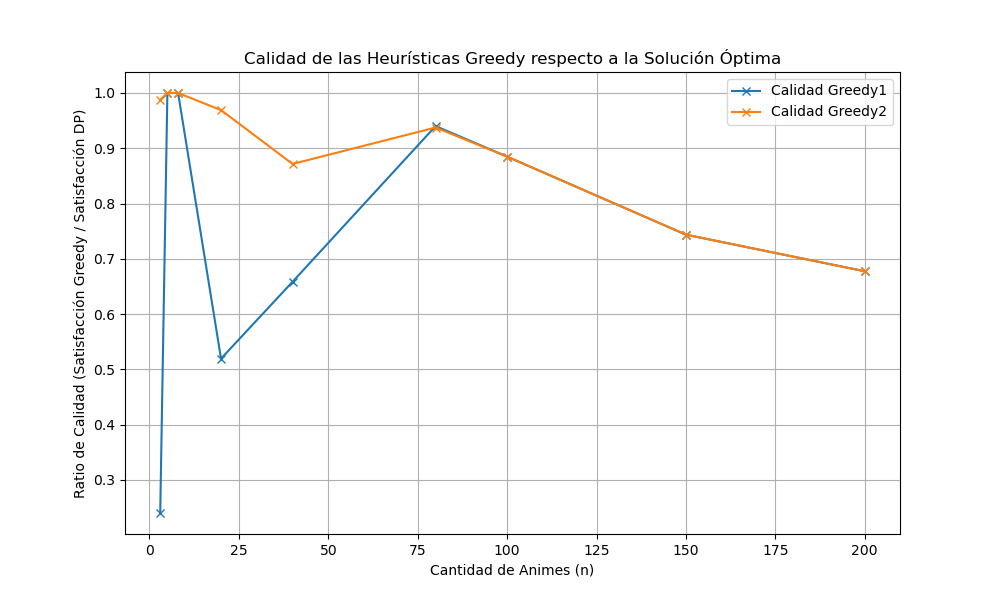
\includegraphics[width=0.8\textwidth]{../code/implementation/data/plots/calidad_vs_n.png}
    \caption{Ratio de calidad de las heurísticas Greedy.}
    \label{fig:calidad}
\end{figure}

Se observa que \textbf{Greedy 2} (Mejor Prefijo Global) tiende a ofrecer mejores resultados que \textbf{Greedy 1} (Siguiente Capítulo), ya que considera el beneficio de completar un anime (bono) de manera más integral al evaluar prefijos completos.
